\chapter{Coordinate System and Reference Frames}\label{ch:coord}
Sonar Workbench uses a right-handed, Cartesian coordinate system known as North-East-Down (NED), as shown in \figname~\ref{fig:NED}. In this coordinate system, the first coordinate, $x$, points north, the second coordinate, $y$, points east, and the third coordinate, $z$, points down. Roll, $\gamma$, is rotation about the $x$ axis, pitch, $\theta$, is rotation about the $y$ axis, and yaw, $\psi$, is rotation about the $z$ axis. The NED coordinate system is ideal for underwater applications, because depth is measured downward from the surface, yaw is measured clockwise from north, and pitch is measured relative to the horizontal plane.

\begin{figure}[!ht]
\begin{center}
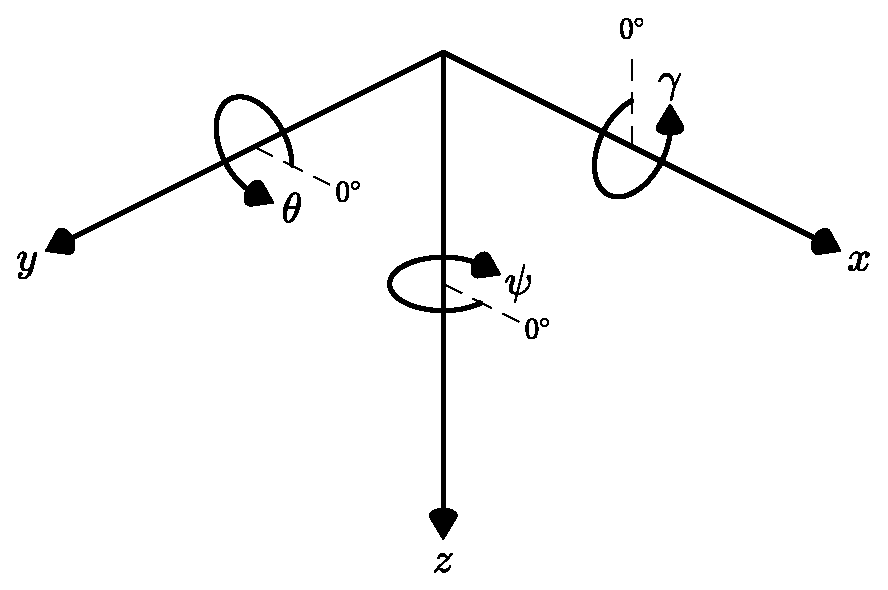
\includegraphics[width=3in]{NEDCoordinateSystem}
\caption{\label{fig:NED}NED coordinate system}
\end{center}
\end{figure}

Sonar Workbench uses three reference frames: the element frame, the array frame, and the body frame. All frames use the NED coordinate system, and each frame can be located relative to another by a combination of translations\footnote{displacement along the $x$, $y$, or $z$ axes} and rotations.

The element frame is always located at the center of the element, with the element's maximum response axis aligned with the $+x$ axis. Exceptions to this alignment are the omnidirectional element, which has no maximum response axis, and the linear element, which the user specifies as initially parallel to one of the three axes ($x$,$y$,$z$) in the element frame. For planar piston elements, the element face lies in the element frame $y$-$z$ plane.

Each element in an array can have arbitrary translation and rotation in the array frame. The array frame origin and orientation is entirely up to the user, but it is typical for planar arrays to be located in center of the array frame's $y$-$z$ plane and for volumetric arrays' geometric center to be located at the origin of the array frame.

The entire array can also be arbitrarily translated and rotated relative to the body frame. For example, a planar array on the nose of a torpedo might have a simple translation along the body frame $x$ axis, while a flank array might have translations along the body $x$ and $y$ axes plus a rotation $\psi$ about the body frame $z$ axis. \figurename~\ref{fig:ReferenceFrames} shows an example of element, array, and body frames for a conformal flank array.

\begin{figure}[!ht]
\begin{center}
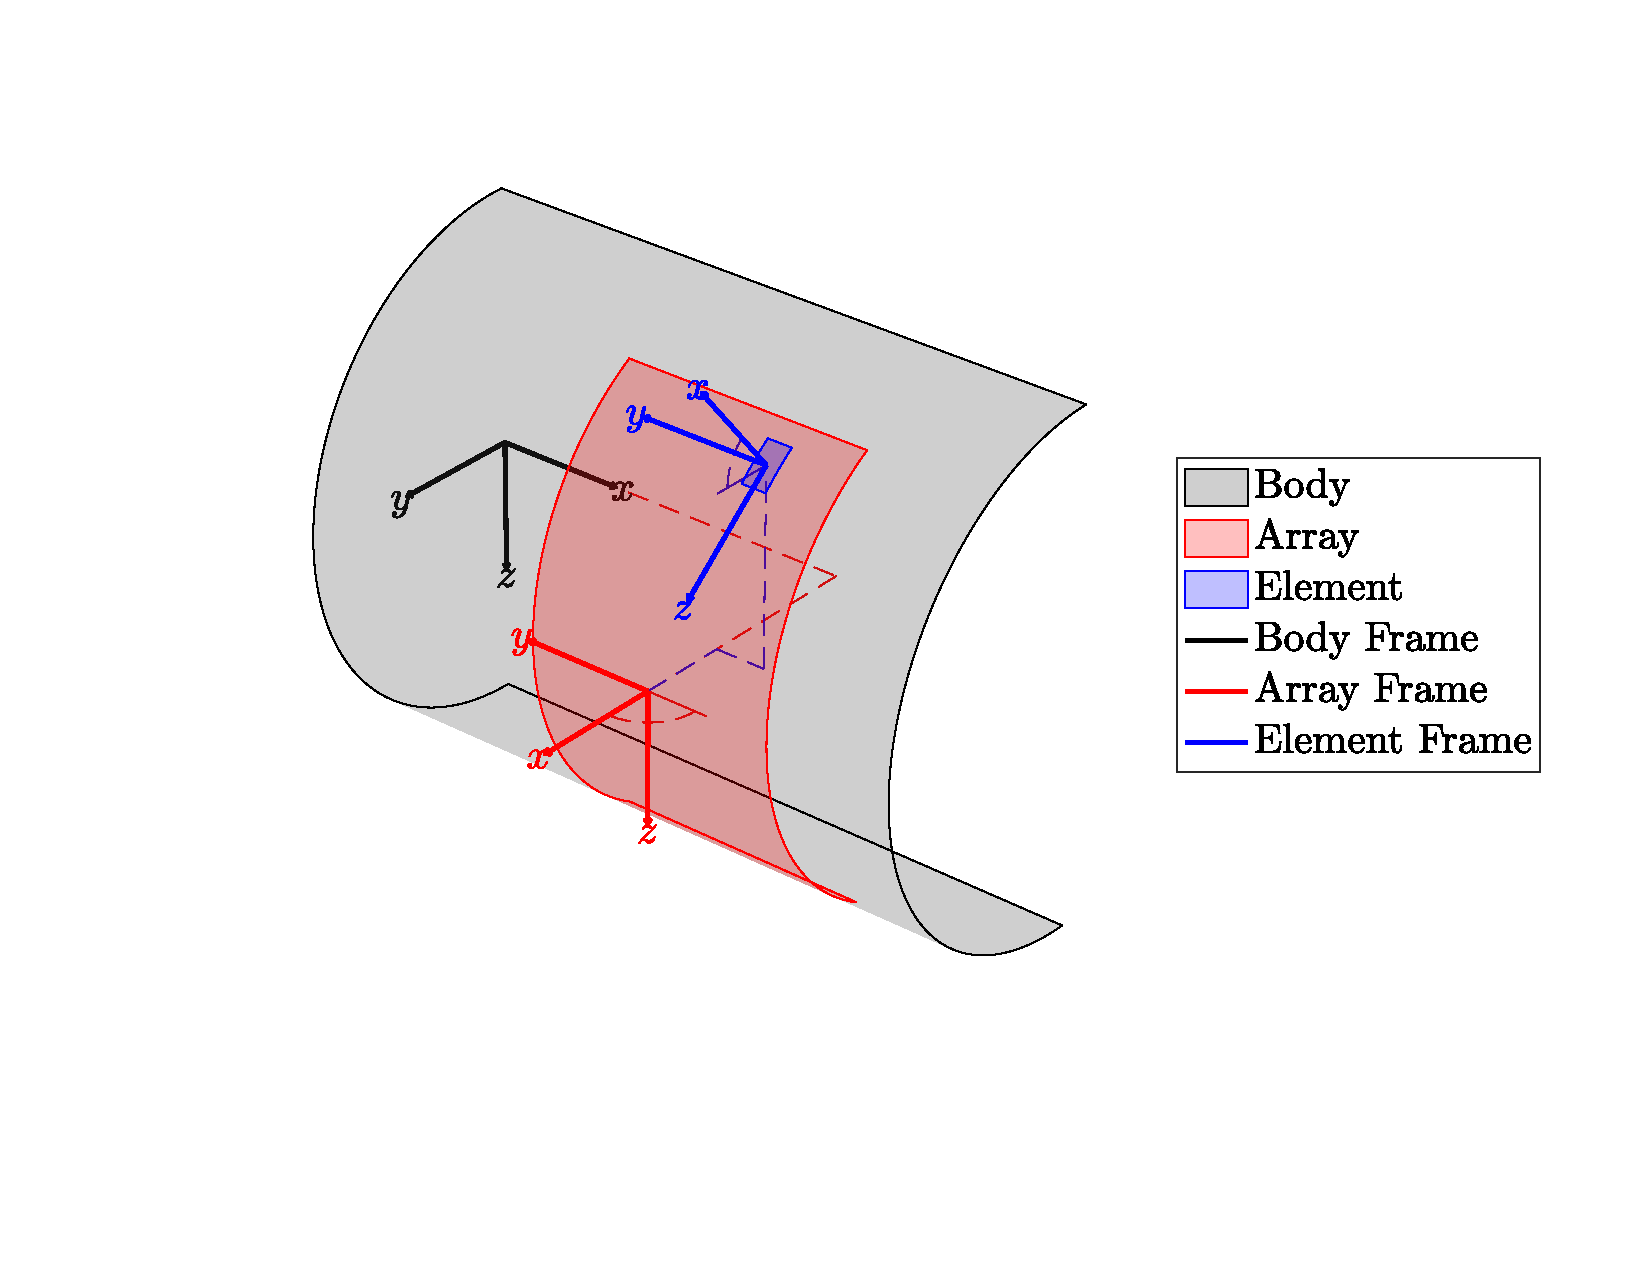
\includegraphics[width=\textwidth]{BodyArrayElementFrame}
\caption{\label{fig:ReferenceFrames}Body, array, and element frames for flank array example}
\end{center}
\end{figure}

Beam patterns are always computed in the body frame as a function of azimuth angles $\psi$ and elevation angles $\theta$. Azimuth and elevation angles are measured from the body frame $+x$ axis. To calculate beam patterns in the array frame, set the array position and orientation vectors to [0;0;0]. More details about element, array, and body frame alignments will be explained in Chapters~\ref{ch:element} and \ref{ch:array}.
